\chapter{Conclusion}

A collection of algorithms was presented which make creating a trajectory for a mobile autonomous drawing robot based on an arbitrary drawing an easy task. While no real world tests have yet been performed with the generated trajectories, comparing the results of the implementation to the manually created drawings shows that the quality of the trajectory is very much comparable, and the manual created drawings have been tested under real world conditions on a beach at the north sea. 

Two different fill algorithms were implemented which produce a fill trajectory for arbitrary input polygons without holes. The spiral fill has also been manually tested on the beach and is known to perform well.

% As shown in the \enquote{A} of the ASL Logo drawing, any polygon with holes can be reduced to a simple polygon. 

This leads to the conclusion that the main goals have been achieved.

The implementation can readily be used to transform arbitrary sketches made, e.g., on a tablet interface with touch input (developed as part of the BeachBot project by Markus Stäuble) for drawing with the BeachBot. Line art generated by other applications (as shown with the font example) can also be used as input, which opens up interesting possibilities for the BeachBot as entertainment device.

The SVG parser works reliably for simple SVG drawings, which covers everything needed for the purpose of the BeachbBot drawings.

% The convex decomposition, used for the Zig Zag fill works good in the general case. 

To conclude, the main work of this thesis has been:

\begin{itemize}
\item Implementing SVG parsing infrastructure to use arbitrary SVG drawings as input
\item Evaluating different fill mechanisms and implementing two algorithms
\item Adapting a generic Travelling Salesman Problem solver for arbitrary, polyline and polygon based drawings
\item Using spiro splines as tool to generate smooth connections between drawing elements
\end{itemize}


%Various drawbacks and suggestions for improvements are made in \autoref{sec:outlook}.

\section{Outlook}\label{sec:outlook}
Of course, the problem is not solved to perfection yet. Several things can be improved and ideas are presented in the following section, that could not be implemented because of time constrains:

\paragraph{Driving over filled areas} The trackmarks are a serious problem for the drawing. While the connection paths can be manually adjusted to not cross through any already filled area, this is tedious and should be automatized. Different possible solutions would be:
\begin{itemize}
\item After an initial run of the TSP algorithm, the solution is examined. If a filled area is crossed over, that specific edge in the distance matrix is assigned a high weight, whereby the connection should not be included when the TSP is solved again. This process is repeated until a solution is found which minimizes the crossings of areas.
\item The intersections of the curved connection paths with already filled areas can easily be found by looking at the convex hulls of the Beziér curve control points that make up the connecting curve (a property of the Beziér curves is that they are always enclosed in the convex hull of the control points). 

If an intersection is evident, the polygon should get an offset which can be calculated by building the Minkowski sum of the polygon and a disk shape of some specified radius.  The offset polygon would be cutted and the appropriate part of that polygon would be added to the curve trajectory (as shown in \autoref{fig:super_conn}).
\item Another possibilty would be to add more $G^2$ spiro control points along the offset polygon which would have to maintain the same minimum distance to each other as defined in the section about smooth connection lines.
\end{itemize}

\begin{figure}
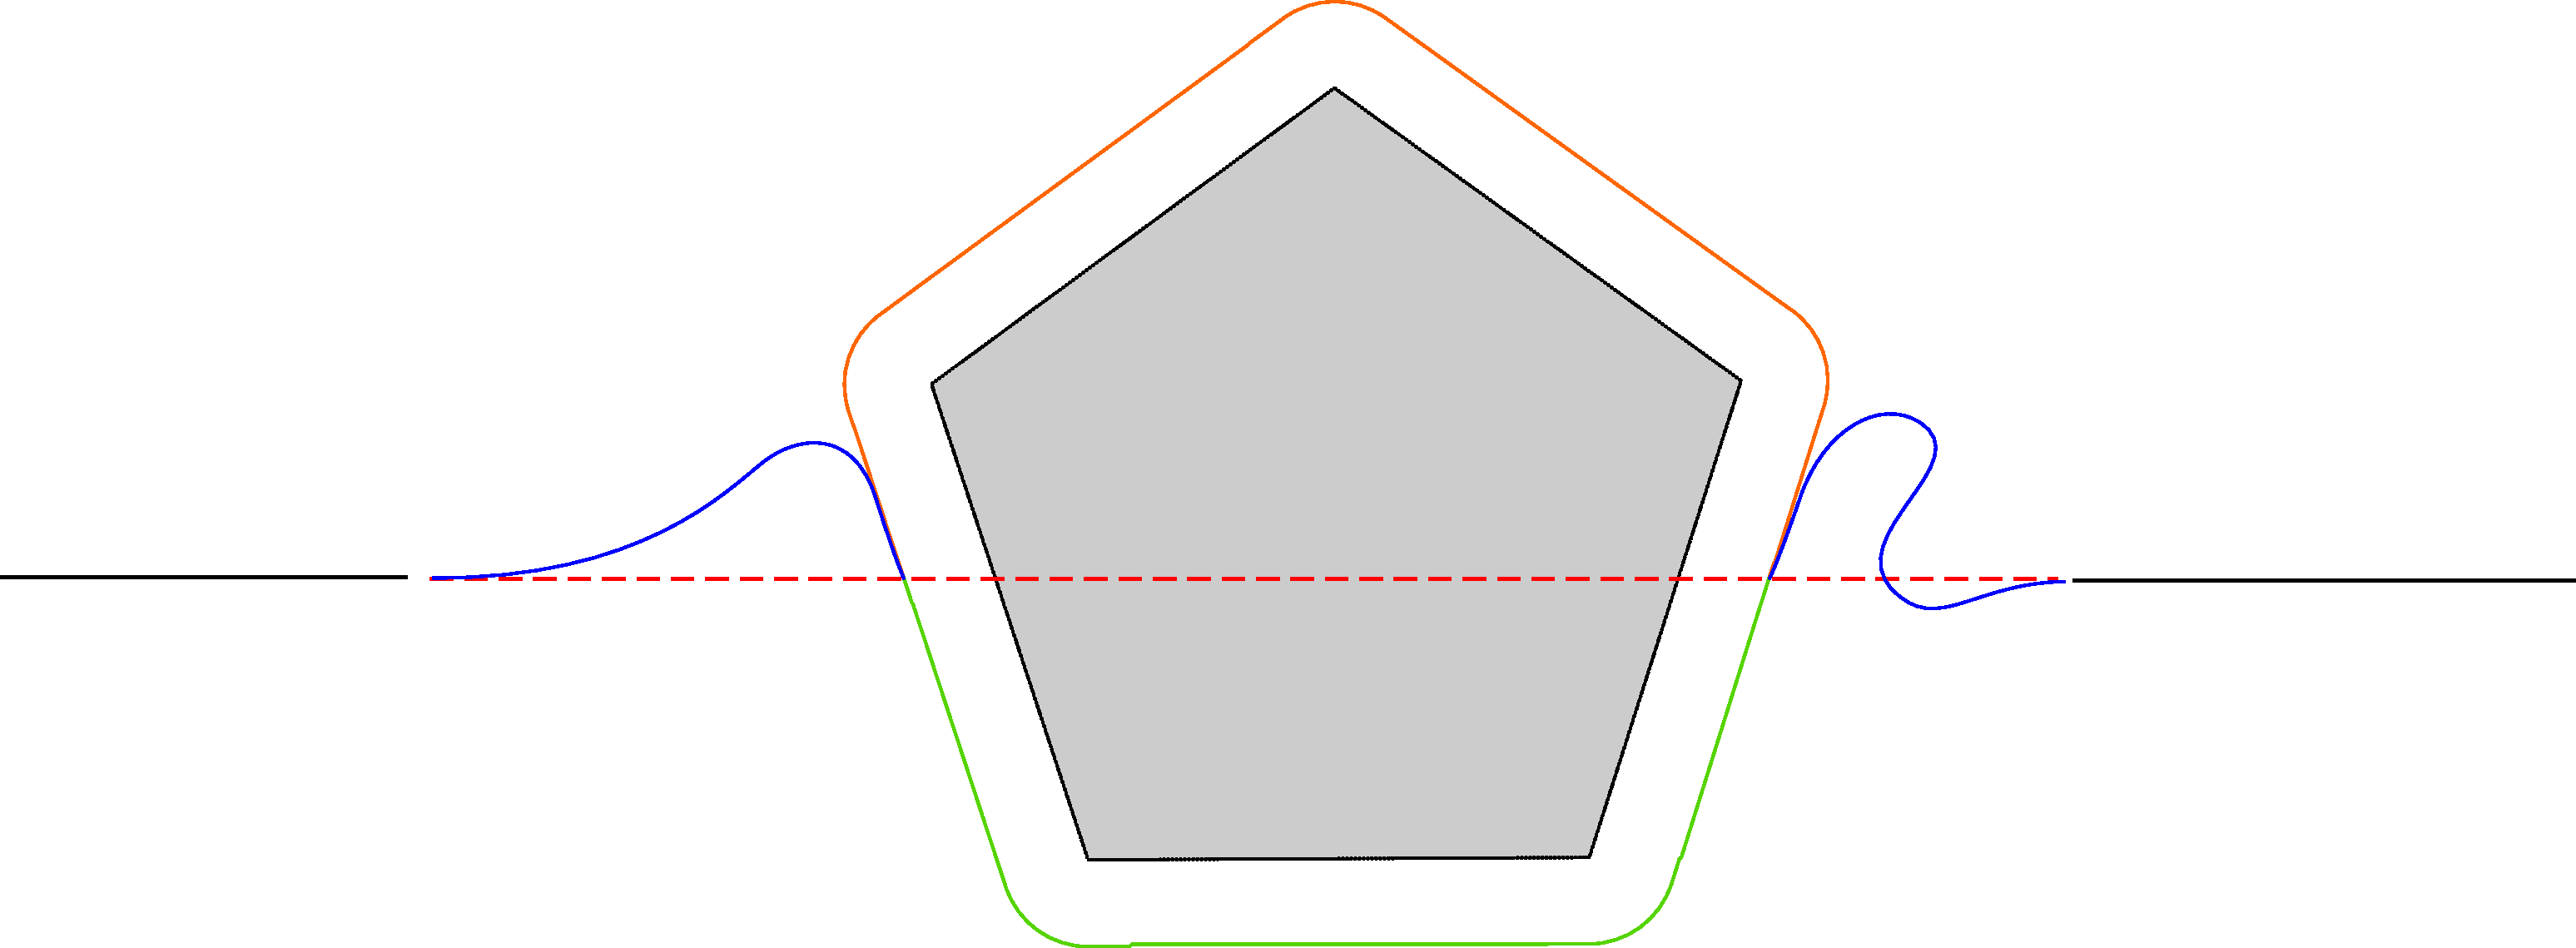
\includegraphics[width=\textwidth]{images/conclusion/minkowski_crossing_avoidance.pdf}
\caption{Using the Minkowski sum to offset the polygon and drive around the filled area (gray). The simple, straight connection is shown in red, the blue connection is the optimized, non-crossing connection.}\label{fig:super_conn}
\end{figure}

\paragraph{Interactive Editing of Spiro Control Points} At the moment, the transition curve between two elements can only be edited in its Beziér representation. Because the Beziér representation of the curve consists of many more points, editing is more difficult then editing the spiro control points (from which there are zero or two per curve). The user interface should include a way to move and add spiro control points. But the control points should keep the distance constraints described in \autoref{sec:smoothspiro} to limit the curvature.

\paragraph{Spiro Connections for Post Processing}

The post processing has one unfortunate drawback if the angle for the outer rounding converges to zero the length of the outer rounding goes to infinity.

To counter this effect and to use a general solution, the post processing step should use the same spiro control point heuristic to create the inner and outer roundings as used for the curvature limited connections. This works well as seen in the \textit{Lion} drawing.

\paragraph{More Robust Heuristic for Spiro Splines}

In the general case the spiro spline heuristic that was used produces good results. However, in some edgecases the numerically obtained solution by the spiro library results in \enquote{Not a Number} values, which is due to erroneous placing of the control points. These edge cases will have to be closely inspected and resolved, for what the time was missing.

\paragraph{Missing Features in the User Interface} Some features are still missing from the user interface due to a lack of time: 

\begin{itemize}
\item Modifying global options such as the rounding radius or the line distance for the Zig Zag fill. These options are currently set per session and read from a configuration file. To change them, the server program has to be restarted.
\item Export and integration with path converter.
\item Post processing is not yet integrated into the user interface
\item The modified transition curves are not sent back to the server
\end{itemize}

All of the improvements are rather minor, but required for a fully functional system.

\paragraph{Polygon with Holes}

Up to now, there was no way found to make the spiral filling algorithm work with polygons with holes, too. 

Polygons with holes can easily be modified to regular polygons by adding cuts from each hole to either another hole or the outer boundary (at least one hole has to have a cut to the outer boundary).

However, the straight skeleton algorithm itself works fine with polygons with holes. Therefore it is possible to generate the inset polygons (all with a constant inset distance of the rake width) and then drive over each polygon, starting from the innermost and traversing to the outside.
The connection between the inset polygons can be made in three different ways:

\begin{itemize}
\item Direct connection to the next outer polygon: for this, the nearest vertex on the next polygon is searched and connected.
\item Direct connection with alternating polygon orientations: If one polygon was oriented clockwise and the other counterclockwise, then the connection between both polygons would resemble the connection of the Zig Zag lines. The connection length would be smaller than in case 1, because the direction has to be changed only once.
\item Connection along the longest edge: the longest edge of the current polygon is searched and diagonally connected to the next polygon (by searching the nearest vertex on the outer polygon and then iterating to the next vertex from there, thus creating a diagonal).

\end{itemize}
All in all polygons for filling are a bit less ideal then the spiral filling because either the connection lines are longer or the polygon is not completely circled.

\paragraph{TSP with respect to real connection distance}

In its current implementation, the distance matrix is filled with the Euclidean distances between the elements. However, after the connection is made, the smooth trajectories are generated, which can be considerable longer, depending on the connection tangents. Therefore, the real connection distances could be used in the distance matrix or the distance could be scaled by a function of the tangent vector angles $\alpha$ and $\beta$.

\paragraph{Better Segmentation of Concave Polygons}

At the moment, the biggest drawback of the optimal convex partitioning algorithm is that the vertices of the convex parts coincide with the vertices of the origin polygon, which sometimes produces unwanted small parts. Finding a polygon partitioning algorithm that splits the polygon into monotone parts might yield better results.

Otherwise, it could also be tried to use the Zig Zag fill without partitioning and connecting the resulting lines with the Travelling Salesman Algorithm.

%\paragraph{Spiral Fill in Sharp Corners} 

%One drawback of the straight skeleton method to create the inset polygons is that the lines in acute angles have a greated distance from each other than in obtuse angles which leaves some areas not properly covered. This can easily be worked around by manually altering the trajectory, but it would still be good to have an automatic solution. 

%The easiest solution would be to reduce the inset width for the inset polygons by some value. The value could either be set empirically or calculated by looking at the straight skeleton, from which the scale factor for the inset distance could be derived.

%\paragraph{Monotone Polygons for Zig Zag Fill}